\chapter{Thème: Système de Lindenmayer}
{ }\hfill\textbf{Niveau:} Avancé\\ \\
\noindent
Dans cette partie, certaines références sont issues:
\begin{itemize}
 \item  de la page Wikipedia sur les L-system: \texttt{http://fr.wikipedia.org/wiki/L-System}.
 \item du livre \og The Algorithmic Beauty of Plants \fg écrit par Przemyslaw Prusinkiewicz et Aristid Lindenmayer.
\end{itemize}
\vspace*{0.5cm}
Cette partie va traiter de la notion de  système de Lindenmayer ou L-system inventé en 1968 par le biologiste hongrois Aristid Lindenmayer. Un L-System est un ensemble de règles et de symboles qui modélisent un processus de croissance d'êtres vivants comme des plantes ou des cellules. Le concept central des L-Systems est la notion de réécriture. La réécriture est une technique pour construire des objets complexes en remplaçant des parties d'un objet initial simple en utilisant des règles de réécriture.\\ \\
Pour ce faire, les cellules sont modélisées à l'aide de symboles. À chaque génération, les cellules se divisent, i.e. un symbole est remplacé par un ou plusieurs autres symboles formant un mot.
\section{Définition formelle}
\noindent
Un L-System est une grammaire formelle qui comprend :
\begin{enumerate}
 \item Un alphabet $V$ : l'ensemble des variables du L-System. $V *$ est l'ensemble des "mots" que l'on peut construire avec les symboles de $V$, et $V +$ l'ensemble des mots contenant au moins un symbole.
 \item Un ensemble de valeur constantes $S$. Certains de ces symboles sont communs à tous les L-System. (Notamment quand on utilisera la tortue).
  \item Un axiome de départ $\omega$ choisi parmi $V +$ , c'est à dire l'état initial.
 \item Un ensemble de règles, noté $P$, de reproduction des symboles de $V$.
\end{enumerate}
Un L-System est alors noté $\{V,S,\omega,P\}$.\\ \\
Considérons le L-system suivant:
\begin{itemize}
 \item Alphabet : $V = \{A, B\}$
 \item Constantes : $S = \{\emptyset\}$
 \item Axiome de départ : $\omega = A$
 \item Régles : $\begin{array}{|l|}
\hline
A \rightarrow AB \\
B \rightarrow A \\ 
\hline
\end{array}
$
\end{itemize}
Les deux règles qui sont données sont les règles de réécriture du système. A chaque étape, $A$ est remplacé par la séquence $AB$, et $B$ est remplacé par $A$. Voici les premières itérations de ce système de Lindemayer:
\begin{center}
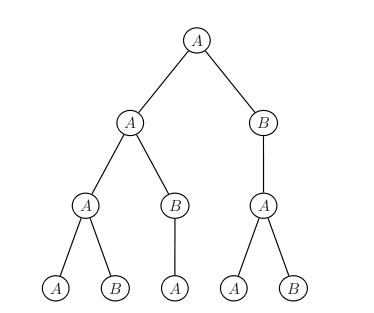
\includegraphics[width=8cm]{images/linden-arbre.png}
\end{center}
\begin{itemize}
\item Itération 1: $A$
\item Itération 2: $AB$
\item Itération 3: $ABA$
\item Itération 4: $ABAAB$
\end{itemize}
\vspace*{0.2cm}
Bien, bien... et concrètement?? Lisons la suite!
\section{Interprétation par la tortue}
\noindent Ce premier exemple vous a permis d'appréhender la notion de système de Lindenmayer sans toutefois peut-être discerner comment nous allons utiliser cela concrètement avec la tortue.\\ \\
C'est là que cela devient intéressant: Chacun des mots ainsi construits ne possède pas de signification particulière. On va alors attacher à chacune des lettres de la séquence, une commande à exécuter par la tortue et générer ainsi des dessins en 2D ou en 3D.
\subsection{Symboles usuels}
\begin{itemize}
 \item [\textbullet] $F$ : Se déplacer d’un pas unitaire ($\in V$)
 \item [\textbullet] $+$ : Tourner à gauche d’angle $\alpha$ $(\in S)$.
 \item [\textbullet] $-$ : Tourner à droite d’un angle $\alpha$ $(\in S)$.
 \item [\textbullet] $\&$ : Pivoter vers le bas d’un angle $\alpha$ $(\in S)$.
 \item [\textbullet] \textasciicircum : Pivoter vers le haut d’un angle $\alpha$ $(\in S)$.
 \item [\textbullet] \textbackslash: Roulez vers la gauche d’un angle $\alpha$ $(\in S)$.
 \item [\textbullet] $/$: Roulez vers la droite d’un angle $\alpha$ $(\in S)$.
 \item [\textbullet] $|$: Effectuer un demi-tour. Avec XLogo: \texttt{td 180}
\end{itemize}
\vspace*{0.2cm}
Prenons par exemple $\alpha=90$ et un déplacement unitaire de 10 pas de tortue, on obtient alors:
\begin{center}
 \begin{tabular}{|c|c|c|c|c|c|c|c|c|}
 \hline
Symbole & $F$ & $+$ & $-$ & $\&$ & \textasciicircum & \textbackslash& $/$ & $|$ \\
 \hline
Commande XLogo & \texttt{av 10}&\texttt{tg 90}&\texttt{td 90}&\texttt{pique 90}&\texttt{cabre 90}&\texttt{rg 90}&\texttt{rd 90}&\texttt{td 180}\\
 \hline
\end{tabular}
\end{center}
\subsection{Flocon de Koch}
Considérons le L-system:
\begin{itemize}
 \item [\textbullet] Etat initial: $F--F--F--$
 \item [\textbullet] Règle de production: $F \rightarrow F+F--F+F$
 \item [\textbullet] Angle $\alpha=60$\degre, le pas unitaire est divisé par 3 entre chaque itération.
\end{itemize}
Premières itérations:
\begin{center}
\begin{minipage}{7.5cm}
 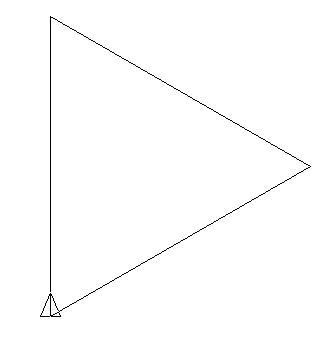
\includegraphics[width=7.5cm]{images/linden-flocon1.png}
\end{minipage}
\begin{minipage}{7.5cm}
 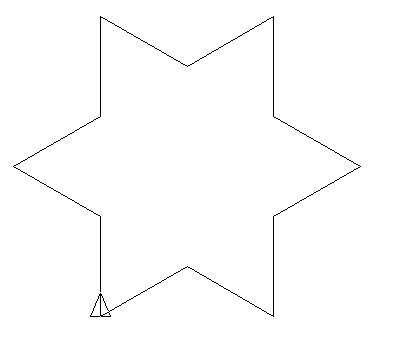
\includegraphics[width=7.5cm]{images/linden-flocon2.png}
\end{minipage}\\
\begin{minipage}{7.5cm}
 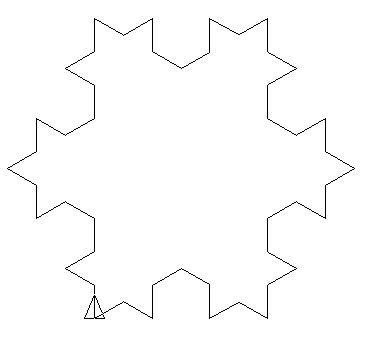
\includegraphics[width=7.5cm]{images/linden-flocon3.png}
\end{minipage}
\begin{minipage}{7.5cm}
 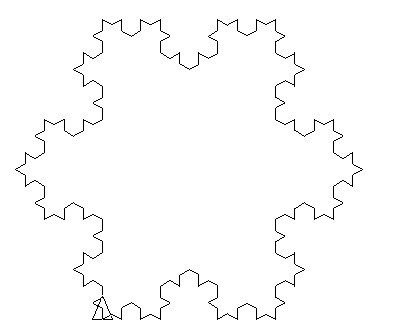
\includegraphics[width=7.5cm]{images/linden-flocon4.png}
\end{minipage}
\end{center}
\noindent Programme en Logo:
\begin{verbatim}
 
pour flocon :p
donne "unit 300/puissance 3 :p-1
repete 3 [F :p-1 td 120]  
fin

pour f :p
si :p=0 [av :unit stop]
F :p-1 tg 60 F :p-1 td 120 F :p-1 tg 60
F :p-1 
fin

\end{verbatim}
\subsection{Courbe de Koch d'ordre 2}
\noindent Intéressons-nous le L-system suivant:
\begin{itemize}
 \item[\textbullet] Etat initial: $F-F-F-F$
 \item[\textbullet] Règle de production: $F\rightarrow F-F+F+FF-F-F+F$
\end{itemize}
Voici les premières représentations en utilisant $\alpha=90$ et en ajustant le pas unitaire de telle sorte que la figure fasse toujours la même taille:
\begin{center}
\begin{minipage}{7.5cm}
 
\includegraphics[width=7.5cm]{images/linden-koch1.png}
\end{minipage}
\begin{minipage}{7.5cm}
 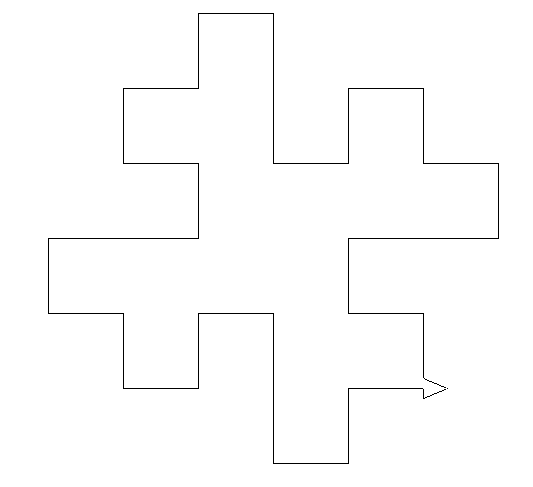
\includegraphics[width=7.5cm]{images/linden-koch2.png}
\end{minipage}\\
\begin{minipage}{7.5cm}
 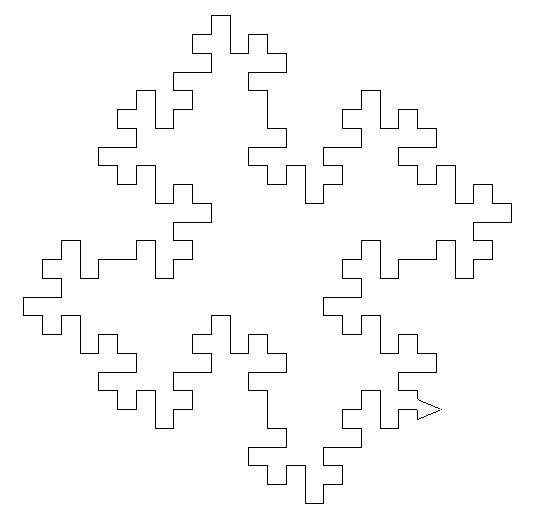
\includegraphics[width=7.5cm]{images/linden-koch3.png}
\end{minipage}
\begin{minipage}{7.5cm}
 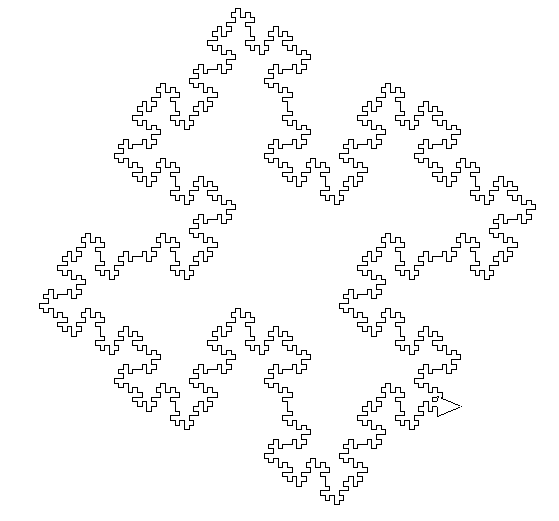
\includegraphics[width=7.5cm]{images/linden-koch4.png}
\end{minipage}
\end{center}
Il est alors très facile de créer le programme Logo permettant de générer ces dessins:
\begin{verbatim}
# p désigne l'itération
pour koch :p
# Entre chaque itération, la distance unitaire est divisée par 4
# Ici, la figure finale aura une taille de 600x600 au maximum
donne "unit 300/puissance 4 :p-1

repete 3 [F :p-1 tg 90] F :p-1 
fin

# La chaine de réécriture
pour F :p
si :p=0 [av :unit stop]
F :p-1 tg 90 F :p-1 td 90 F :p-1 td 90
F :p-1 F :p-1 tg 90 F :p-1 tg 90 F :p-1 td 90 F :p-1
fin
\end{verbatim}
\subsection{Courbe du dragon}
\begin{itemize}
 \item[\textbullet] Etat initial: $F$\\
 \item[\textbullet] Règle de production: $\begin{array}{|l|}
\hline
A\rightarrow A+B+ \\
B\rightarrow -A-B \\
\hline
\end{array}$ 
\end{itemize}
\begin{verbatim}
pour a :p
si :p=0 [av :unit stop]
a :p-1 tg 90 b :p-1 tg 90
fin

pour b :p
si :p=0 [av :unit stop]
td 90 a :p-1 td 90 b :p-1

fin

pour dragon :p
donne "unit 300/8/ :p  
a :p
fin
\end{verbatim}
\begin{center}
 \begin{minipage}{7cm}
 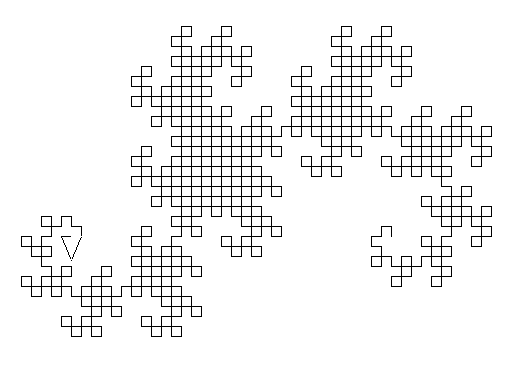
\includegraphics[width=7cm]{images/linden-dragon10.png}
 \begin{center}
  \texttt{dragon 10}
 \end{center}
\end{minipage}
 \begin{minipage}{7cm}
 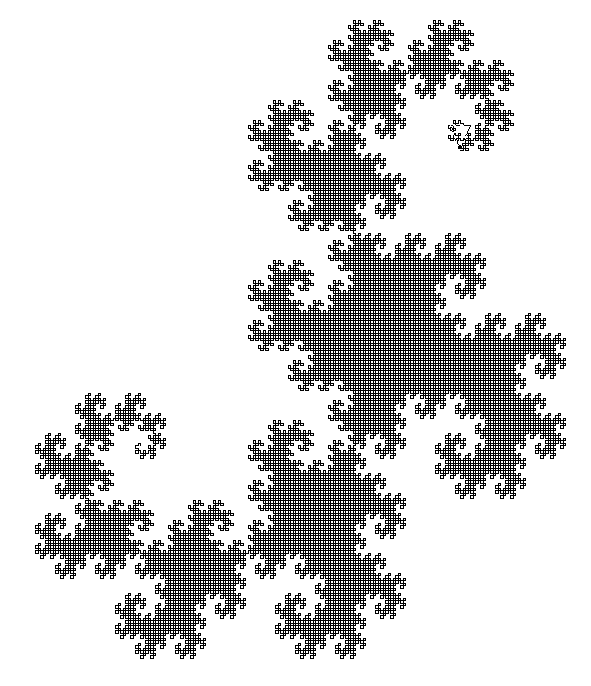
\includegraphics[width=7cm]{images/linden-dragon15.png}
 \begin{center}
  \texttt{dragon 15}
 \end{center}
\end{minipage}
\end{center}

\subsection{Courbe de Hilbert en 3D}
\noindent L'exemple suivant traite de la courbe de Hilbert dans l'espace, c'est une courbe qui a la propriété de remplir parfaitement un cube quand on augmente le nombre d'itérations.\\ \\
Voici le L-system associé:
\begin{itemize}
 \item Etat initial: $A$
 \item Angle $\alpha=90$\degre, on divise la longueur unitaire par deux à chaque itération.\\
 \item Règle de production: $\begin{array}{|l|}
\hline
A\rightarrow B-F+CFC+F-D\&F \textrm{\textrm{\textasciicircum}} D-F+\&\&CFC+F+B// \\
B\rightarrow A\&F\textrm{\textrm{\textasciicircum}} CFB\textrm{\textasciicircum} F \textrm{\textasciicircum} D\textrm{\textasciicircum} \textrm{\textasciicircum}-F-D\textrm{\textasciicircum}|F\textrm{\textasciicircum} B|FC\textrm{\textasciicircum} F\textrm{\textasciicircum} A// \\
C\rightarrow|D\textrm{\textasciicircum}|F\textrm{\textasciicircum} B-F+C\textrm{\textasciicircum} F\textrm{\textasciicircum} A\&\&FA\&F\textrm{\textasciicircum} C+F+B\textrm{\textasciicircum} F\textrm{\textasciicircum} D// \\
D\rightarrow|CFB-F+B|FA\&F\textrm{\textasciicircum} A\&\&FB-F+B|FC// \\
\hline
\end{array}$
\end{itemize}
\begin{verbatim}
pour hilbert :p
ve perspective
donne "unit 400/puissance 2 :p
lignedef ftc :unit/2
a :p
lignefin
vue3d
fin

pour a :p
si :p=0 [stop]
b :p-1 td 90 av :unit tg 90  c :p-1 av :unit c :p-1
tg 90 av :unit td 90 d :p-1 pique 90 av :unit cabre 90 d :p-1
td 90 av :unit tg 90 pique 180 c :p-1 av :unit c :p-1
tg 90 av :unit tg 90 b :p-1 rd 180
fin

pour b :p
si :p=0 [stop]
a :p-1 pique 90 av :unit cabre 90 c :p-1 av :unit b :p-1 cabre 90 
av :unit cabre 90 d :p-1 cabre 180 td 90 av :unit td 90 d :p-1 cabre 90 
td 180 av :unit cabre 90 b :p-1 td 180 av :unit c :p-1 cabre 90 av :unit 
cabre 90 a :p-1 rd 180 
fin

pour c :p
si :p=0 [stop]
td 180 d :p-1 cabre 90 td 180 av :unit cabre 90 b :p-1 td 90 av :unit tg 90 
c :p-1 cabre 90 av :unit cabre 90 a :p-1 pique 180 av :unit a :p-1 pique 90 
av :unit cabre 90 c :p-1 tg 90 av :unit tg 90 b :p-1 cabre 90 av :unit cabre 90 
d :p-1 rd 180 
fin

pour d :p
si :p=0 [stop]
td 180 c :p-1 av :unit b :p-1 td 90 av :unit tg 90 b :p-1 td 180
av :unit a :p-1 pique 90 av :unit cabre 90 a :p-1 pique 180 av :unit
b :p-1 td 90 av :unit tg 90 b :p-1 td 180 av :unit c :p-1 rd 180
fin
\end{verbatim}
Et les premières itérations obtenues:
\begin{center}
\begin{minipage}{7cm}
 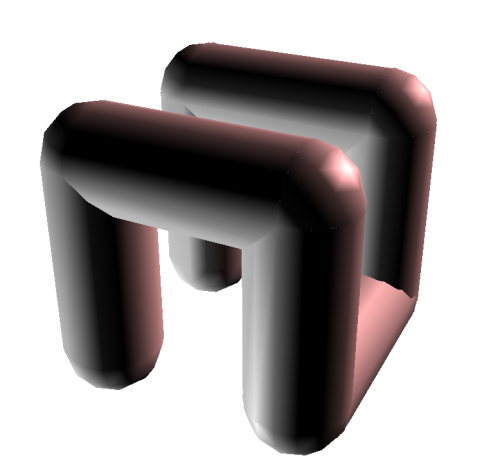
\includegraphics[width=7cm]{images/linden-hilbert1.png}
\end{minipage}
\begin{minipage}{7cm}
 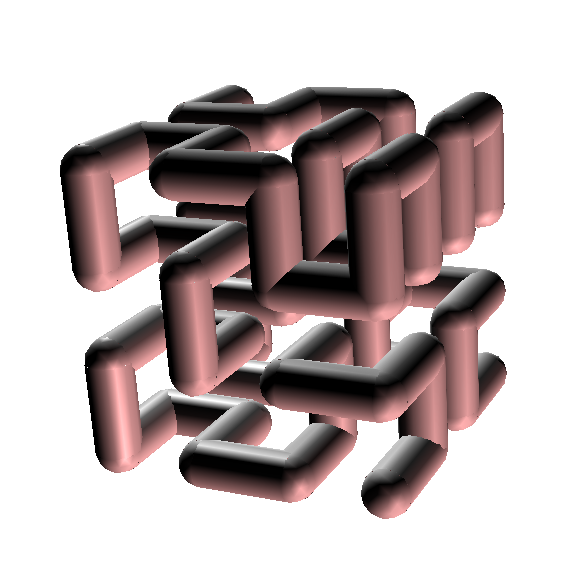
\includegraphics[width=7.5cm]{images/linden-hilbert2.png}
\end{minipage}\\
\begin{minipage}{7cm}
 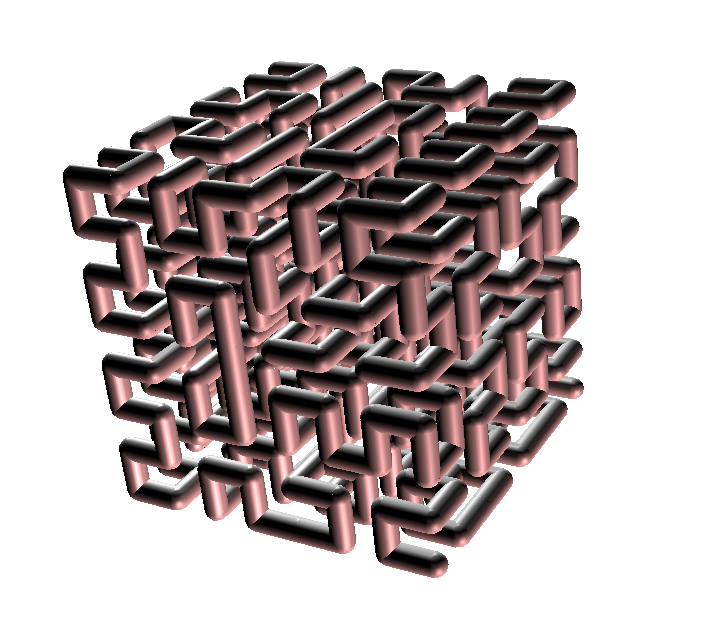
\includegraphics[width=7cm]{images/linden-hilbert3.png}
\end{minipage}
\begin{minipage}{7cm}
 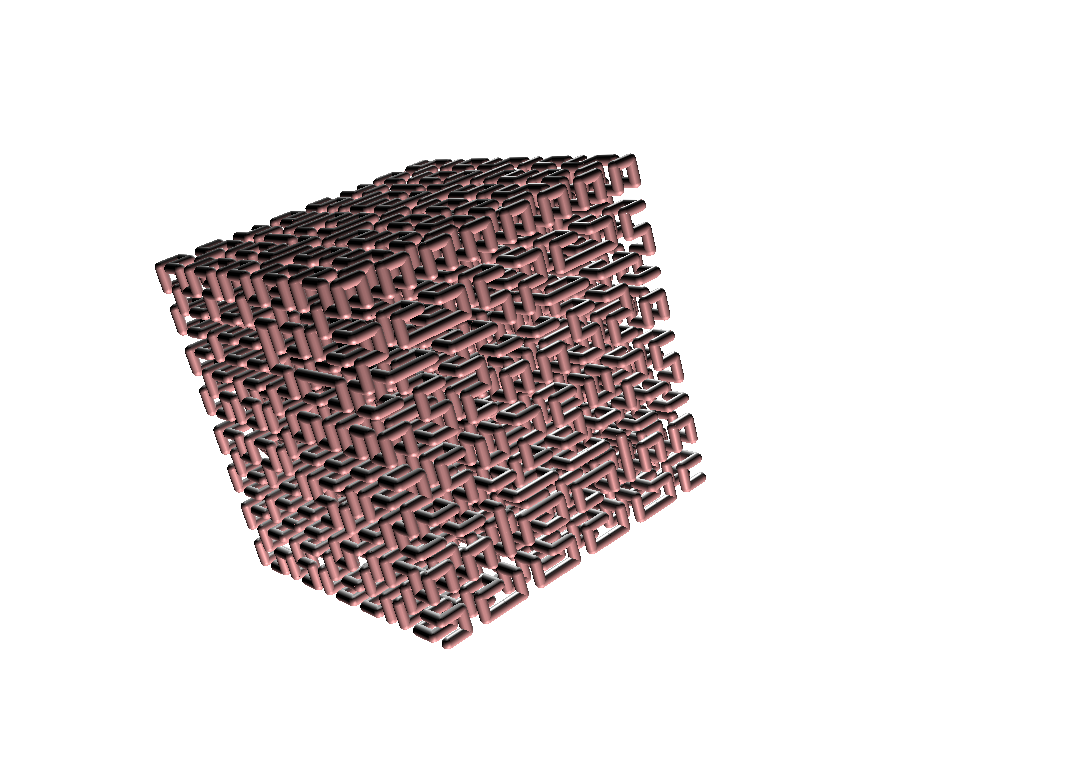
\includegraphics[width=9cm]{images/linden-hilbert4.png}
\end{minipage}
\end{center}